%==========================================================================
% Capítulo 1: O que é LaTeX?
%==========================================================================
\chapter{O que é \LaTeXX} 
\label{cap:LaTeX}

Esse capítulo é um pouco polêmico!
Alguns provavelmente falarão que não precisaria abordae tais tópicos em um 
minicurso de 3\unit{h}, vist que poderíamos ser mais diretos e realizarmos 
logo a prática. 
Entretanto, entendo que é um tópico importante, que definirá algumas ideias 
sobre o que é o \LaTeXX, bem como se propõe a uma abordagem mais atual dos 
recursos disponibilizados para composição tipográfica. 
Penso que, se eu soubesse dessas coisas logo na minha iniciação no \LaTeXX, 
teria uma visão bem mais consistente de seu uso. 

% seção 01 ================================================================

\section{Como se fala \LaTeXX?}
\label{sec:como-se-fala}

Pode até ser irrelevante essa informação, mas é sempre bom conhecermos as 
coisas corretamente, não? 

Sei que vocês sabem que não estamos falando daquela seiva da árvore que é 
usada para produzir diferentes materiais como tinta, luvas, etc. 
Ou seja, não estamos falando do Látex. 

O \LaTeXX\ não é Látex. 
Nem na ideia, nem na pronúncia. 

Existem duas maneiras aceitáveis para pronunciar o nome em questão: uma mais
voltada ao inglês e outra mais ``abrasileirada''. 

Antes de exibir a pronúncia, entretando, vamos conhecer a pronúncia da 
palavra \TeX.
Não é \textit{Téckis}, mas \textit{Téc} (como em ``\textbf{tec}nologia''). 
Isso se deve ao fato de que a palavra \TeX, na realidade, veio da junção 
das três letras gregas: {\grega τ} (tau);\, {\grega ε} (épsilon); e, 
{\grega χ} (chi --- lê-se \textit{Qui}, como em ``\textbf{Qui}abo'').
Essas letras gregas, juntas e em maiúsculas, ficam: {\grega ΤΕΧ}; mas o 
idealizador dessa linguagem de programação, como veremos, denominada \TeX, 
simplesmente quis modificar a disposição do {\grega Ε} para mostrar que se 
trata de algo relacionado à tipografia.

A tipografia é a arte e o processo de criação na composição e impressão de um 
texto, física ou digitalmente (Wikpédia).

É interessante notarmos que a palavra \TeX\ está relacionada à 
\textsf{tecnologia}, visto que é uma linguagem de programação; mas também 
relacionada à \textsf{arte}, visto que a tipografia é descentende da 
\textit{Caligrafia} --- uma arte que resiste ao tempo e traça muitos parâmetros para formas elegantes de letras/fontes.
Isso não é ao acaso!
A palavra \TeX\ foi escolhida justamente porque as palavras \textsf{arte} 
({\grega τεχνη}) e \textsf{tecnologia} ({\grega τεχνολογία}) possuem a mesma raiz linguística {\grega τεχ}. 

Do exposto, agora podemos indicar as formas aceitáveis de pronunciar a palavra\LaTeXX.

\begin{itemize}
  \item[\emoji{speaking-head}] Se você quiser pronunciar mais parecido com o        Inglês, fale ``\textit{LeiTéc}''. 
  \item[\emoji{speaking-head}] Mas, se quiser falar mais abrasileirado, use 
        ``\textit{LaTéc}''.
  \item[\emoji{prohibited}] Apenas, evite, depois desse minicurso, falar 
        ``\textit{LaTéckis}''; ou, pior ainda, ``\textit{LáTeckis}''. \emoji{winking-face-with-tongue}
\end{itemize}

% seção 02: Mas, o que é o LaTeX ==========================================

\section{Já sei falar, mas o que é \LaTeXX?}
\label{sec:word-latex}

Tudo bem\ldots\
Como vocês já sabem pronunciar corretamente a essa palavra, vamos agora
dizer \ldots\ o que \textbf{não} é \LaTeXX. 

Calma, mas alguns, no início, costumam comparar o \LaTeXX\ com algum editor 
de textos, como o Word ou LibreOffice. 
O \LaTeXX\ não é um editor de textos!
E, mesmo que fôssemos comparar, a filosofia seria diferente!
Editores como Word ou LibreOffice são \textsf{WYSIYYG} (\textit{What You See Is What You Get} --- O que você vê é o que você tem); ou seja, se você 
quer um símbolo como $\sum$, você precisa clicar sobre ele em algum lugar
do editor.
Na filosofia do \LaTeXX, você digita comandos e depois é necessário uma 
\textit{compilação}, para que os símbolos (e o próprio texto) sejam 
exibidos adequadamente.

Então, já temos uma ideia do que \textbf{não} é o \LaTeXX!
Não é um editor de textos!
E, por conta disso, é natural que curva de aprendizado seja um pouco 
diferente: é necessário uma aquisição prévia de vocabulários para comandos. 
Entretanto, espera-se uma flexibilidade e otimização de tarefas tipográficas
à medida que esse vocabulário é expandido, principalmente quando o texto 
que se deseja produzir é complexo (com \textit{hiperlinks}; referências 
cruzadas; referências bibliográficas; index; muitas figuras ou tabelas; 
etc.). 
Veja a Figura~\ref{fig:latex-vs-word} para essa comparação hipotética. 

\begin{figure}[!htbp]
  \centering
    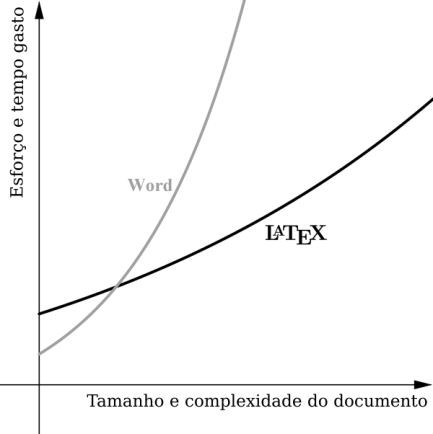
\includegraphics[width=0.7\textwidth]{latex-vs-word}
  \caption{Curva de aprendizado}
  \label{fig:latex-vs-word}
\end{figure}

Vocês estão percebendo que o \LaTeXX\ está parecendo uma espécie de 
\textsf{linguagem}, visto que há uma aquisição de vocabulário, estruturas 
e organização. 
Mas, que tipo de ``linguagem'' seria o \LaTeXX?

% subsection 03: TeX vs LaTeX ---------------------------------------------

\subsection{\TeX\ vs \LaTeXX}
\label{subsec:tex-latex}

Para entender que tipo de linguagem é o \LaTeXX, precisamos conhecer o que 
é o \TeX. 

Tudo começou quando 
\href
{
  https://en.wikipedia.org/wiki/Donald_Knuth
}
{
  \sffamily
  Donald Ervin Knuth
}
recebeu uma cópia de seu novo livro de programação. 
Ele simplesmente não se conformou com o resultado tipográfico em suas mãos. 
Como cientista da computação Knuth pensou que poderia criar uma linguagem 
de programação que preenchesse harmoniosamente, com algum algorítmo 
engenhoso, com o ``0'' (zero), para espaços onde \textbf{não há} ``tinta'';
e, ``1'' (um) para espaços \textbf{com} tinta.
Foi formada a idea do \TeX, no final dos anos 70. 

A linguagem \TeX\ produzia comandos primitivos essenciais, mas 
ainda era preciso criar um conjunto de ``atalhos'' (macros) para certas 
estruturas de um texto, por exemplo. 
O próprio Knuth produziu esse conjunto de macros, inicialmente, denominado 
\textsf{Plain \TeX}.
Mas, ao que parece, esse conjunto de macros ainda dava muito trabalho para 
ser usado! \emoji{sweat-smile}

Foi, então, que, em 1985, Lamport criou um conjunto de macros muito especial: \LaTeXX. 
Facilita nossa vida até hoje!
Lembrem-se disso: 

\tcboxC{
  \sffamily
  O \LaTeXX\ veio para facilitar nossa vida!
}

Entretando, não nos enganemos: o \LaTeXX\ não é uma simples linguagem de 
marcação! 
Ele é um sistema de preparação de documentos, em alta qualidade tipográfica.
